


\subsection{Resultat diskussion}
% måske nævne noget omkring vertikale fejl i højdemodellen 
På baggrund af resultaterne er der en række elementer der kan diskuteres. Resultaterne fra Inundation Modellen til at simulere 2023-stormfloden har været fornuftigt. To af studieområderne, Gedser Havn og Hesnæs, har haft simulerings resultater der er tæt afspejler det observerede data (figur \ref{Figur: Målt & simuleret Gedser} og \ref{Figur: Målt & simuleret Hesnæs}). For Geder Havn og Hesnæs har Inundation modellen været mindre i udstræk end det observeret data. \\
Aabenraa og Præstø derimod har haft henholdsvis et større og mindre areal oversvømmet i Inundation Modellens resultat end det der skete under stormfloden grundet en række eksterne faktorer der skete under selve stormfloden.\\

For Aabenraa er forskellen mellem det observeret data og simuleringen forårsaget af en række beredskabs tiltag der blev implementeret langs havnen i løbet af den 20. oktober 2023 (figur \ref{Figur: Beredskabstiltag}). Dette har inkluderet en ca. 1 km lang watertube og barrikader af BigBag sandsække langs vejen ved havnen. Det sorte kryds i figur \ref{Figur: Beredskabstiltag} indikerer hvor watertuben bristede på grund af vandpresset. På trods af dette brist formåede det lokale beredskab Brand og Redning Sønderjylland at få lavet en dæmning af sække med jord der hindrede vandets strømning mod syd og længere ind i Aabenraa midtby og dermed det bagvedliggende område der blev oversvømmet i Inundation Modellens resultat i figur \ref{Subfig: Model Aabenraa}. \\
\begin{figure}[H]
    \centering
    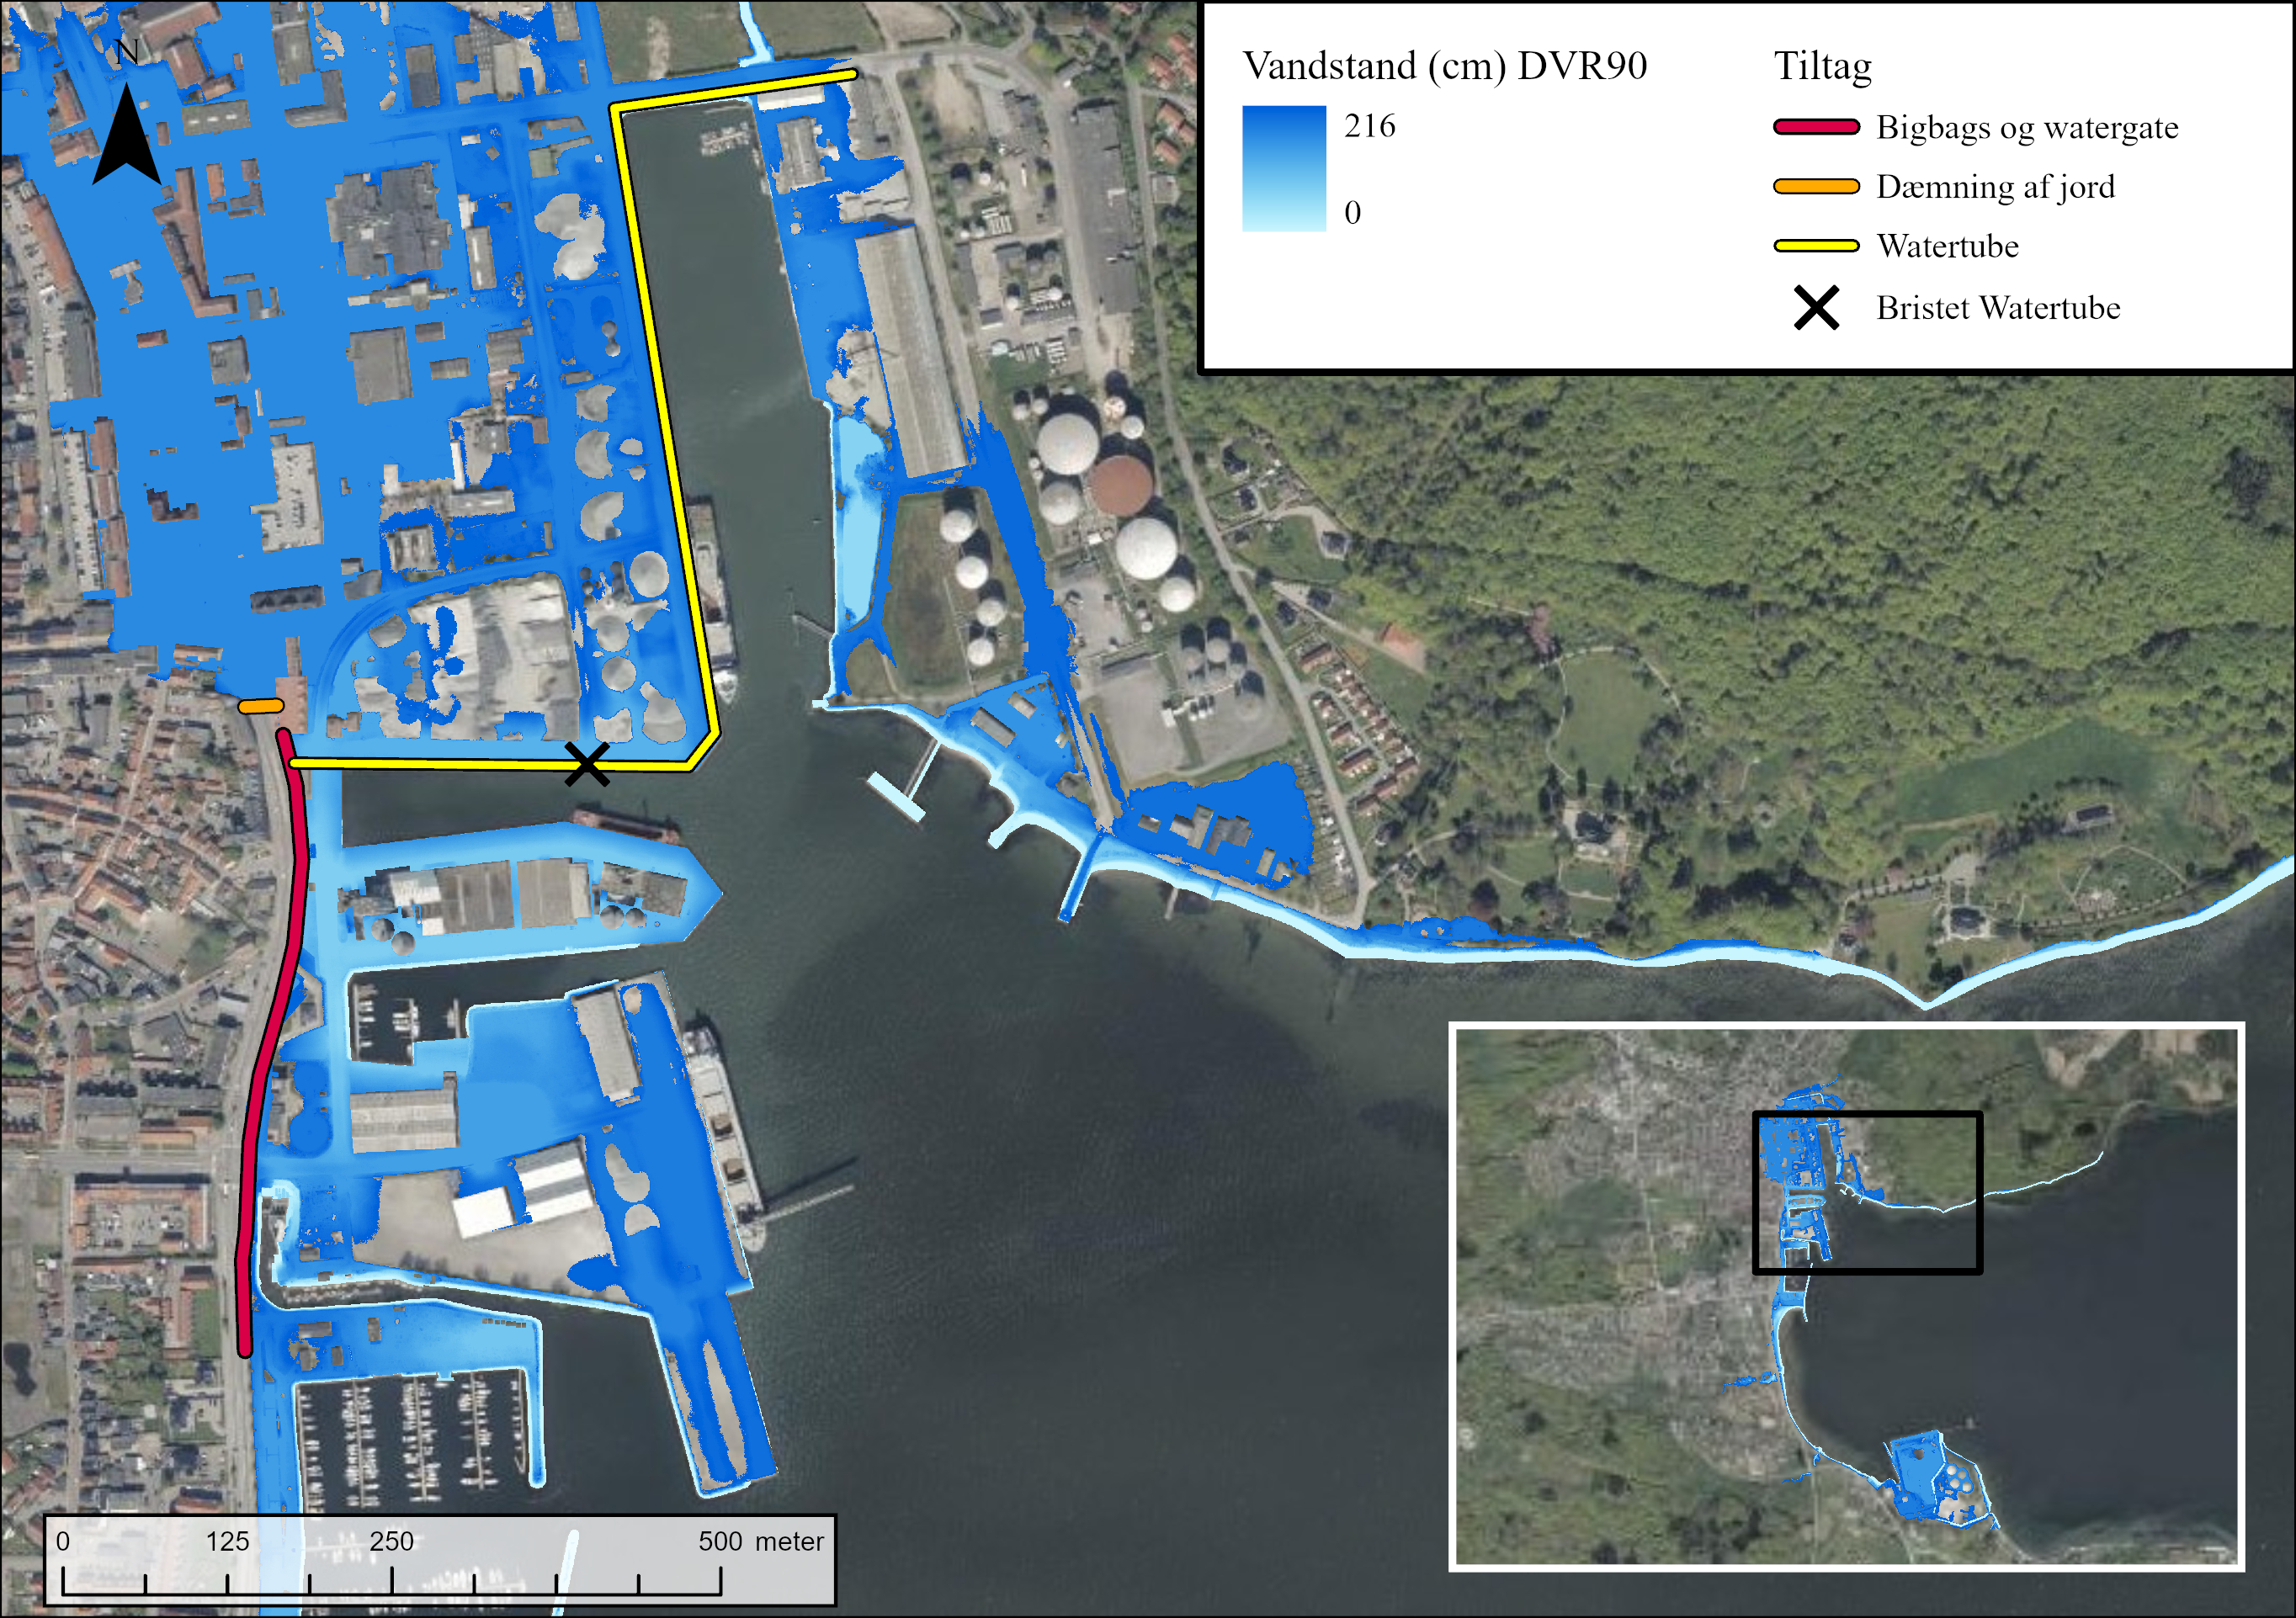
\includegraphics[width=0.8\linewidth]{images/diskussion/beredskabstiltag.jpg}
    \caption{Kort over beredskabstiltag foretaget i løbet af den 20. oktober 2023 i Aabenraa og den observeret oversvømmelse. Dæmningen af jord blev etableret efter watertuben bristede. Kilde: Aabenraa Kommune}
    \label{Figur: Beredskabstiltag}
\end{figure}
Udover dette har der været to områder i det observeret data er der blev konstateret oversvømmelse, men hvor modellen ikke indikerede en oversvømmelse. De to områder er to mindre vandløb mellem Aabenraa by og Ensted Industrihavn og noget af det bagvedliggende areal (figur \ref{Figur: Tilpasnings fejl}). Denne forskel skyldes sandsynligvis en datafejl i kortet fra Aabenraa Kommune. 
\begin{figure}[H]
    \centering
    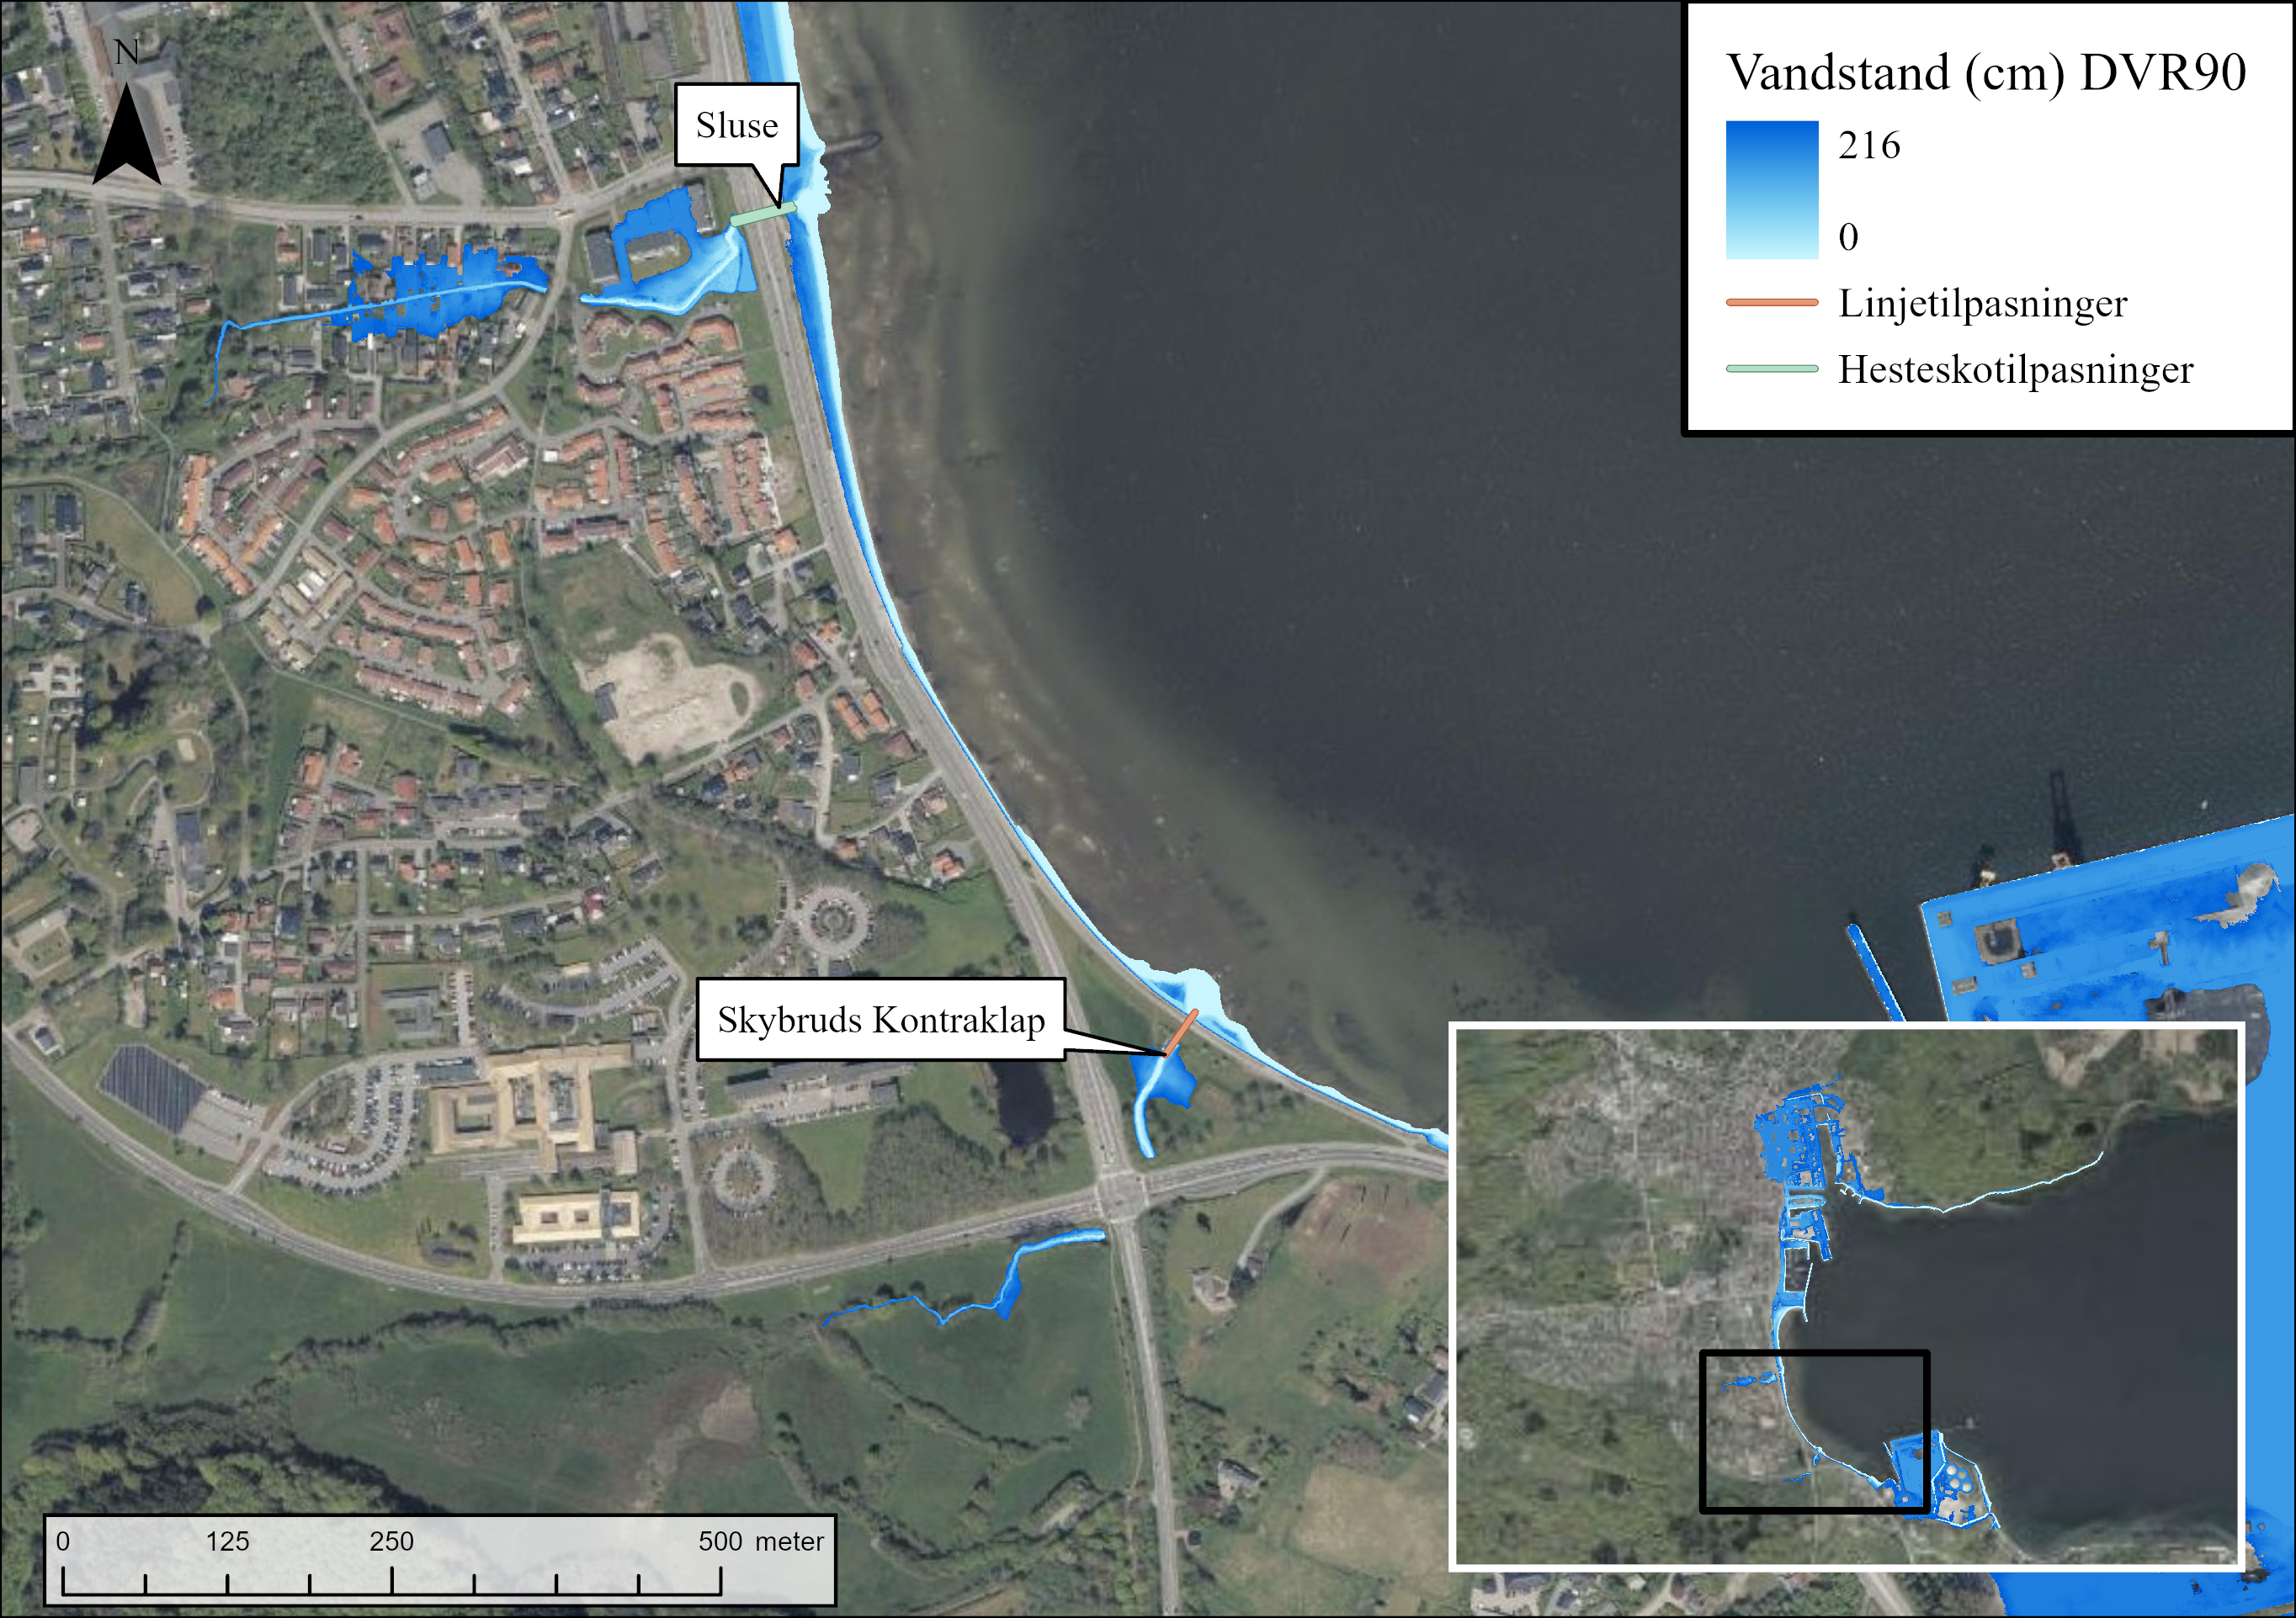
\includegraphics[width=0.8\linewidth]{images/diskussion/tilpasnings_error.jpg}
    \caption{Kort over to hydrologiske tilpasninger der ved fejl ikke er implementeret korrekt i kortet modtaget fra Aabenraa Kommune.}
    \label{Figur: Tilpasnings fejl}
\end{figure}
Begge vandløb har en udmunding ud til fjorden. Den nordligste tilpasning er en hesteskotilpasning, med en klassifikation fra GeoDanmark som en højvandssluse. Denne ville have været lukket under stormfloden, og der er ingen observationer om at denne sluse brød sammen under stormfloden. Den anden tilpasning længere sydpå er en kontraklap til at føre vand væk fra landet til havet under et skybrud. Begge objekter er aktuelle og aktive fra 2015, så antagelsen om ændret brug må forkastes. Det er derfor mere sandsynligt at de to hydrologiske tilpasninger er blevet glemt at inkludere i datasættet, da andre lignende tilpasninger er blevet korrekt implementeret eller at vandet på anden vis er trængt ind over. \\  

I Præstø har den primære forskel mellem det observeret data og simuleringen været forårsaget af sammenbruddet af sluseporten ved udmundingen af Tubæk Å. Dette resulterede i at Tubæk Ådal og dele af byen blev oversvømmet. Dette er ikke blevet fanget af Inundation Modellen, da det er en uforudset hændelse. Det kan derfor diskuteres hvorvidt den observeret oversvømmelse og modellen ville være mere ens hvis sluseporten ikke brød sammen. \\
Samtidig kan det diskuteres om der blev lavet barrikader længere opstrøms af Tubæk Å, da oversvømmelseskortet fra Vordingborg Kommune stopper abrupt når åen passerer under en vej syd for byen. Der er ikke noget der indikerer at vandet er blevet bremset under denne vej og det må derfor at antages at kommunen ikke har lavet undersøgelser af oversvømmelsesniveauet forbi dette punkt. \\

% arealanvendelse 
Til kvantificeringen af påvirkede arealanvendelser blev der foretaget en reklassifikation af arealklasserne præsenteret i BaseMap fra \cite{Jepsen_levin_2013, levin_basemap04_2022}. Det primære formål med reklassifikationen var at reducere antallet af arealklasser for overskuelighedens skyld samt en filtrering af nødvendige klasser såsom søer, vandløb, hav osv. Reduktionen af arealklasser har derfor betydet at kvantificeringen af påvirkede arealer er blevet mindre transparent og mere generaliseret i det endelige resultat. I tilfældet med Aabenraa og Præstø hvor det simulerede resultat varierede fra det observerede data, ville de originale 35 klasser kunne beskrive mere detaljerede og specifikke forskelle i påvirkede arealanvendelser end de otte overordnede klasser. \\
Desuden blev der udregnet en procentvis andel af det totale oversvømmede areal til at visualisere hvor meget oversvømmet areal hver klasse udgjorde det samlede areal. Dette har været misvisende som set i figur \ref{Figur: Påvirket arealanvendelse Præstø} hvor naturområder i Præstø for det simuleret resultat har en højere andel oversvømmet af det totale areal, men det svarer til et mindre areal i hektar end det observeret data. \\ 


Simuleringerne af fremtidige stormfloder i form af statistiske 100-års hændelser og fremskrivningen af 2023-stormfloden har været fornuftige. Da resultatet af 100-års hændelsen er direkte fra DMI er resultatet her det forventede. Fremskrivningen af stormfloden er derimod det mere interessante. Fremskrivningen blev baseret på medianværdien af IPCCs projektioner for 2030 samt DMIs forventede vandstandsniveau ved udgangen af det 21. århundrede. Denne metode indebar en vis usikkerhed, idet den forudsætter, at havspejlsstigningen siden 1995 har været lineær. Her er det værd at bemærke at denne usikkerhed ikke umiddelbart kan dokumenteres, da \cite{danish_meteorological_institute_dmi_2024} ligeledes antager den samme lineær udvikling. Det er derfor væsentligt at understrege at denne udregning forudsætter at stigningen er lineær og det derfor ikke nødvendigvis afspejler observeret data og ligeledes ikke er tilfældet alle steder i verden. \\
Uanset denne antagelse har fremskrivningen af stormfloden resultateret i fornuftige værdier, der ikke er urealistiske for lokaliteten og for det SSP scenarie de blev beregnet på. \\


\subsection{Inkluderingen af bygninger i DHyM}
En af de prominente metodiske overvejelser, der blev taget relativt tidligt i arbejdsprocessen var at inkludere bygninger i den digitale hydrologiske model (DHyM), som ikke passerbare enheder i terrænet. Denne beslutning blev truffet ved at argumentere for at vand ikke kan passere direkte igennem bygninger, når en oversvømmelse sker og for at sætte et ens datagrundlag for at kunne sammenligne Inundation Modellens resultat med det modtaget data fra kommunerne. Dertil er det ikke en normal procedure at tilføje bygninger til en DHyM \citep{khosh_bin_ghomash_technical_2024}, da der ofte bruges en DTM til hydrologisk modellering fremfor en digital overflade model (DSM), som inkluderer bygninger og træer. Derudover fjernes muligheden for potentielle undersøgelser og analyser af stormfloders påvirkning på bestemte bygninger og bygningstyper samt vurderinger af bygningers risici ved fremtidige oversvømmelser ved at tilføje bygninger til DHyM. Dette har været tilfældet ved denne undersøgelse. \\
Derudover blev alle bygninger tildelt den samme højdeværdi på 20 meter. En mere nøjagtig fremgangsmåde ville have været at udregne den maksimale taghøjde af bygningerne for at sikre korrekt repræsentation af virkeligheden, men da denne undersøgelse primært har fokuseret på at vandet ikke skulle kunne passere igennem en bygning har dette ikke været en prioritet. \\


\subsection{Begrænsninger ved Inundation Modellen}
Inundation Modellen har været et godt redskab til simulere oversvømmelsesudbredelsen ved bestemte vandstandsniveauer og været fornuftigt til at simulere den stormflods hændelse der skete i oktober 2023. 
Den største fordel modellen har, er dens brugervenlighed og dens relative simple struktur. Dette gør det nemt for individuelle personer, studerende og organisationer at anvende modellen. Dertil er det en fordel at modellen opererer i et GIS-regi og kan dermed kombineres med andre geospatiale data, såsom arealanvendelsesdata i dette projekt, men også andet punkt-, linje- og polygondatasæt for at undersøge risici ved oversvømmelser på sektorer og samfundskritisk infrastruktur. Modellen er også relativ hurtig i simuleringstid, hvis den hardware den udføres på er god. Simuleringstiden for resultaterne i dette projekt har været samlet 16 timer og 45 minutter og har derfor potentielt været en del længere end hvis modellen blev udført på kraftigere hardware. Simuleringstiden må forventes at kunne mere end halveres hvis hardwaren er kraftigere.\\

Derudover er der flere værktøjer i Inundation Modellens pakke, som ikke er blevet anvendt i dette projekt, herunder et værktøj der kan bestemme hvor vandet trængte ind og dermed identificere sårbare lokaliteter, der kan bruges i kommunernes planlægning af kyst- og stormflodssikring. I kombination med dette værktøj kan Inundation Modellen igen køres for aedt tjekke hvorvidt implementeringen af stormflodssikring har haft en effekt. Koblet med at modellen også er relativ hurtig i simuleringstid er dette en arbejdstilgang der kan være brugbar for både kommuner og private.\\


På trods af dette er der derimod også en række begrænsninger ved modellen. Modellen er en 100\% statisk numerisk model og det betyder derfor at der ikke er mulighed for at inkorporere en tidslig faktor. Mange stormfloder sker over en periode på ca. en til to døgn og det betyder dermed at vandmasserne ikke oversvømmer hele arealet på ingen tid, som modellen indikerer. Denne manglende tidsskala gør også at modellen ikke tager højde for korrekt hydrodynamisk adfærd, hvor det vil tage længere tid for en vandmasse at passere igennem mindre passager, såsom rør, og kortere tid igennem bredere passager, såsom under broer.\\

Andre aspekter som modellen ikke tager højde for inkluderer bl.a. effekten af vind, bølgeskvulp og regn. Modellen leverer derfor kun et overblik over hvor oversvømmelserne sker på baggrund af vandstandshøjden. Hvis der derfor er et beskyttende dige langs en kyststrækning, der er højere end vandstandsniveauet, så vil det ikke blive oversvømmet i modellen, hvorimod i en virkelig stormflodshændelse er det muligt at bølger og vind vil presse vandet ind over diget og dermed oversvømme det bagvedliggende område. I samme bane er modellen ikke egnet til at håndtere sammensatte oversvømmelser (\textit{eng.} compound flooding), hvor områder oversvømmelses fra nedbør og havet samtidig, da oversvømmelsen beregnes fra en kilde der placeres ude i havet. Dette er områder hvor kraftigere og mere avanceret modeller såsom Deltares Super-Fast Inundation of Coasts (SFINCS) og DHIs MIKE21/3 er i stand til at simulere.\\

Modellen kræver dertil data af høj kvalitet. Den digitale terrænmodel (DTM) skal være i høj opløsning med en lille cellestørrelse \citep{seenath_effects_2018, williams_geographic_2022} for at være mere virkelighedstro samt omfattende data af hydrologiske tilpasninger er også krævet for at modellen kan simulere korrekt hydrologisk bevægelser i terrænet \citep{bales_sources_2009}. Er DTM og hydrologiske tilpasninger enten utilstrækkelige eller ikke tilstede vil det have indflydelse på kvaliteten af modellens resultat og i forlængelse modellens anvendelighed. \\

Derudover er modellen lige nu eksklusiv til ArcGIS Pro softwaren. Det betyder at modellen fungerer godt i det specifikke miljø og kan derfor nemt integreres med andre dele af Esris ArcGIS miljø, såsom ArcGIS Online, Enterprise og Field Maps, til at arbejde i felten med stormflodssikring og på tværs af samarbejdspartnere. At være begrænset til Esris ArcGIS-miljø betyder derfor også at modellen er låst bag en stejl betalingsmur især for kommercielt brug og er dermed udenfor potentiel brug fra danske kommuner og andre private interessenter, der ikke har mulighed for at imødekomme den høje pris. En løsning til dette vil være at udvikle et lignende værktøj der fungerer i et gratis open-source GIS produkt såsom QGIS. \\



% hvad gør modellen godt 
% hvad gør modellen knap så godt
% hvilke forbedringer kan implementeres?
% andre begrænsninger



  

% Udregningen af fremskrevet stormflod og relaterede usikkerheder

% something something konfidensinterval maybe?



% hvor kunne den bruges
% hvilke klienter
% hvordan kunne det implementeres
% er der begrænsninger for noget af dette